\documentclass[10pt, conference, compsocconf]{IEEEtran}

\usepackage[bookmarks=true]{hyperref}
\usepackage{epsfig}
\usepackage{amsmath,amssymb,amsfonts,latexsym}
\usepackage{enumerate}
\usepackage{xspace}
\usepackage{epsf,picinpar}
\usepackage{varioref}
\usepackage{colortbl,multirow,hhline}
\usepackage{listings}
\usepackage{amssymb}
\usepackage{colortbl,multirow,hhline}
\usepackage{algorithmic}
\usepackage{algorithm}
\usepackage{caption}
\usepackage[normalem]{ulem}
\usepackage{xcolor}
\usepackage{pifont}
\usepackage{xcolor,colortbl}
\usepackage{url}
\usepackage{balance}
\usepackage{graphicx, subfigure}
\usepackage{longtable}
\usepackage{lscape}
\usepackage{multirow}
\usepackage{listings}
\usepackage{framed}
\usepackage{morefloats}
\usepackage[T1]{fontenc}
\usepackage{array}
\usepackage{pdfpages}
\usepackage{fancybox}
\usepackage{amsmath}
\usepackage{flushend}
\usepackage{booktabs}
\usepackage{enumitem}
\usepackage{gensymb}

\renewcommand{\ttdefault}{cmr}

\newcommand{\limit}[1]{\textcolor{red}{\ding{46}~Page limit:~#1}\\}
\newcommand{\todo}[1]{\textcolor{blue}{\ding{46}~#1}} 
\newcommand{\ie}{\emph{i.e.,}\xspace}
\newcommand{\eg}{\emph{e.g.,}\xspace}
\newcommand{\etc}{etc.\xspace}
\newcommand{\etal}{\emph{et~al.}\xspace} 

\graphicspath{{./figures/}}
    
\begin{document}

\title{
	\todo{Smart Fire Alarm system using AADL and Acceleo}
}

\author{
\IEEEauthorblockN{Renan Greca}
\IEEEauthorblockA{
renan.greca@gssi.it}
\and
\IEEEauthorblockN{Maria Teresa Rossi}
\IEEEauthorblockA{
mariateresa.rossi@gssi.it}
}

\maketitle

\begin{abstract}
\todo{Technology can be a useful tool to decrease the damage caused by fires. In this assignment, a model for a smart fire alarm system using the Architecture Analysis and Design Language is proposed. Analysis is performed on the model in order to estimate the time it takes for a control center to receive an alarm signal and dispatch emergency services. Furthermore, an alternative structure to the model is proposed, and the advantages and disadvantages between the two approaches are considered. Finally, an Acceleo template is presented, providing an example of how the model could be used to generate web pages including components and subcomponents of the system.}
\end{abstract}

\begin{IEEEkeywords}
Empirical Software Engineering, Fire Detection, System Modeling and Analysis, Code Generation
\end{IEEEkeywords}

\section{Introduction}
%This document represents a template of the assignment of the course \textit{Immigration to software systems and services} at the GSSI\cite{gssi}.

%The total length of this document must not exceed 20 pages, including references, appendixes, \etc

%In this section you have to provide (i) the informal description of the system you are going to model (ii) the main motivation behind the AADL analysis you chose, (iii) brief description of the obtained results, and (iii) brief description of your Acceleo program.  

In the United States, over 3,000 people per year lose their lives to fires \cite{usfiredeaths}. Technology can be a powerful tool to reduce this number and increase the safety of buildings and their inhabitants. In this assignment, we propose a model of a smart fire alarm system, as well as analysis of certain aspects of the model and an example of tool that could be developed with the model.

In order to detect fires and alert the appropriate authorities, this system is formed of sensors, communication devices, infrastructure, an alarm and a database. In broad terms, environmental data is obtained by the sensors, which is sent to the mobile phones of local users and to a remote control center, which can analyze the data and dispatch emergency services. The model for this system is developed using the Architecture Analysis and Design Language (AADL) \cite{aadl}, which allows us to model hardware and software aspects of a multi-device system.

Considering the time sensitive nature of fire detection, prevention and combat, we decided that the latency of the system, that is, the time it takes for data to be sent from one component to another, is the most important aspect to be analyzed. Using OSATE \cite{osate}, a tool developed for AADL development, latency analysis was performed on the model, measuring time between production and consumption of data from different devices. The analysis reports were used to display and understand the latency of the system.

Finally, the model is used as basis for an Acceleo \cite{acceleo} project which produces a web page displaying components from the system.

The remainder of this document is organized as follows: chapter 2 explains the AADL model produced; chapter 3 proposes an alternative structure to the model and shows the analysis results; chapter 4 elaborates on the Acceleo template used to generate a web page using the AADL model as input; finally, chapter 5 provides final thoughts on the assignment.

%\limit{1}
\section{Part 1 -- Architecture}

%Describe the model you created.
%Here you will describe the identified architecture, the chosen design decisions, the relevant information about the produced models, such as smart solutions applied, how you organized the architectural specification in a modular way, \etc

The primary goal of our AADL model was to specify components of the Smart Fire Alarm system with enough detail to provide a reasonable estimate of data transmission latency between relevant devices. To do this, we organized elements of the network into three layers: (1) the top layer, which describes three sub-networks; (2) the middle layer which describes the physical devices forming each sub-network; and (3) the bottom layer describing internal details of some of these devices.

The first layer is formed by three sub-networks. The Sensor Network contains devices connected using short-ranged wireless communication technologies (Wi-fi, Bluetooth and Zigbee) and, in a real-world implementation, would be placed within the same house or building. The Communication Network provides a very high-level abstraction of the infrastructure that allows the connection between two remote locations over the Internet. Finally, the Control Center is also a high-level abstraction of the location where sensor data is gathered for analysis and also where an alarm signal is received if it is necessary to dispatch emergency services.

\autoref{fig:smartfirealarm} shows a broad overview of the system and how the three sub-networks connect to each other. The Sensor Network connects to the Communication Network through two ports, depending on which communication technology is used, and data is then forwarded into the Control Center over a wired Internet connection.

%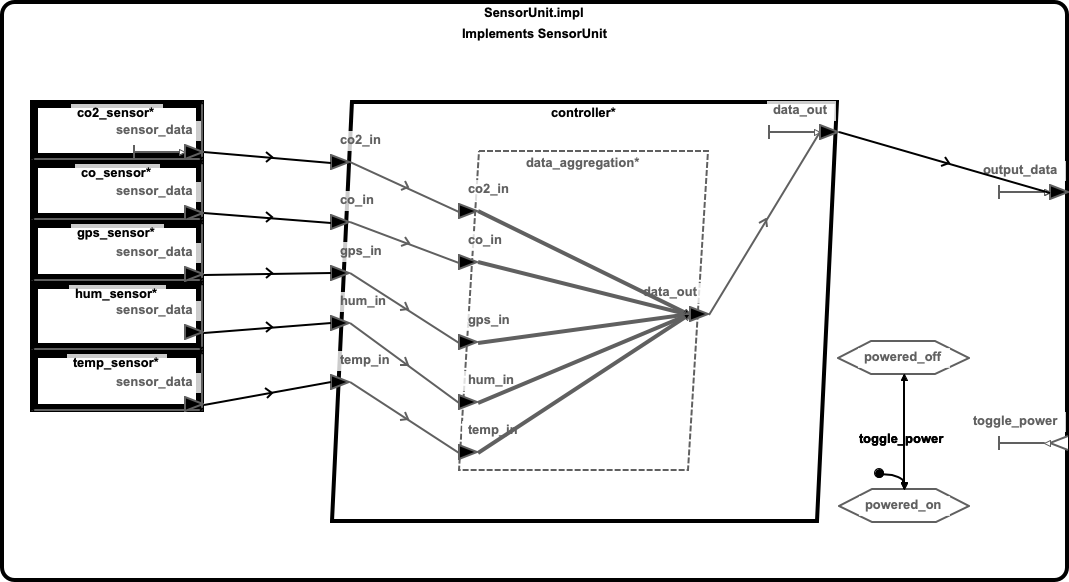
\includegraphics[width=\textwidth]{SensorUnit.png}

\begin{figure*}[h]
\caption{General structure of the system}
\label{fig:smartfirealarm}
\centering
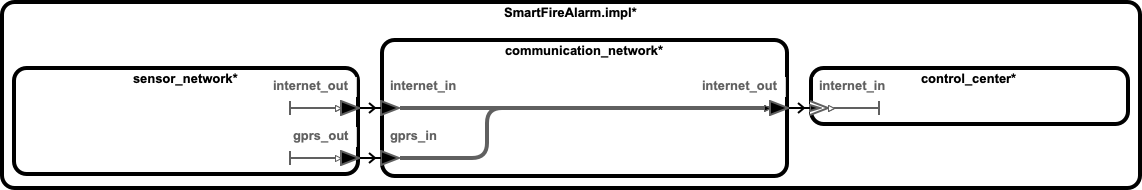
\includegraphics[width=0.9\textwidth]{SmartFireAlarm}
\end{figure*}

\begin{figure*}[h]
\caption{Structure of the Sensor Network}
\label{fig:sensornetwork}
\centering
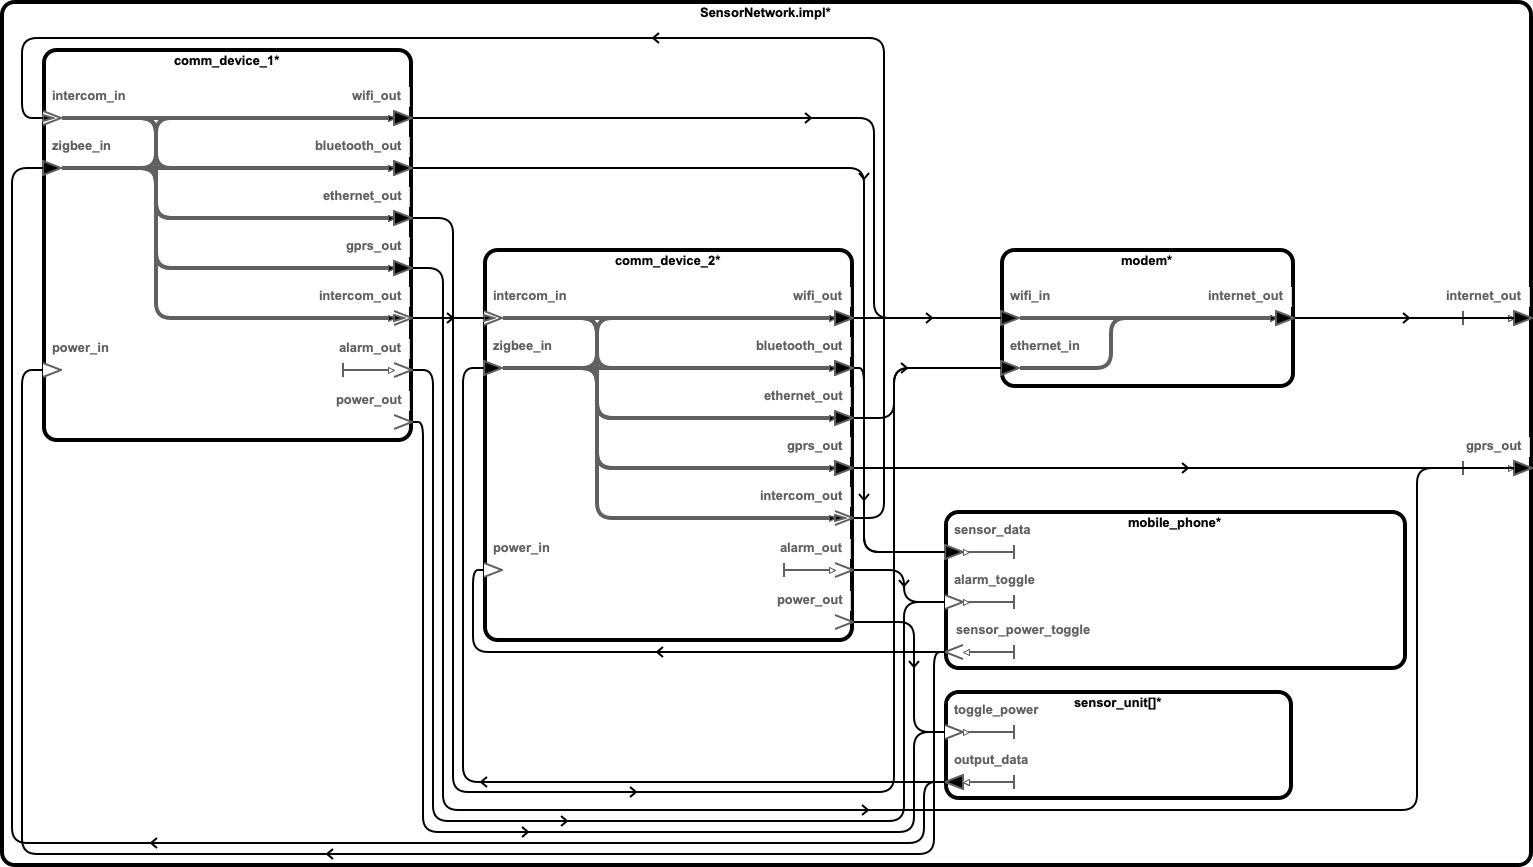
\includegraphics[width=0.9\textwidth]{SensorNetwork}
\end{figure*}

\begin{figure*}[h]
\caption{Internal structure of a Sensor Unit}
\label{fig:sensorunit}
\centering
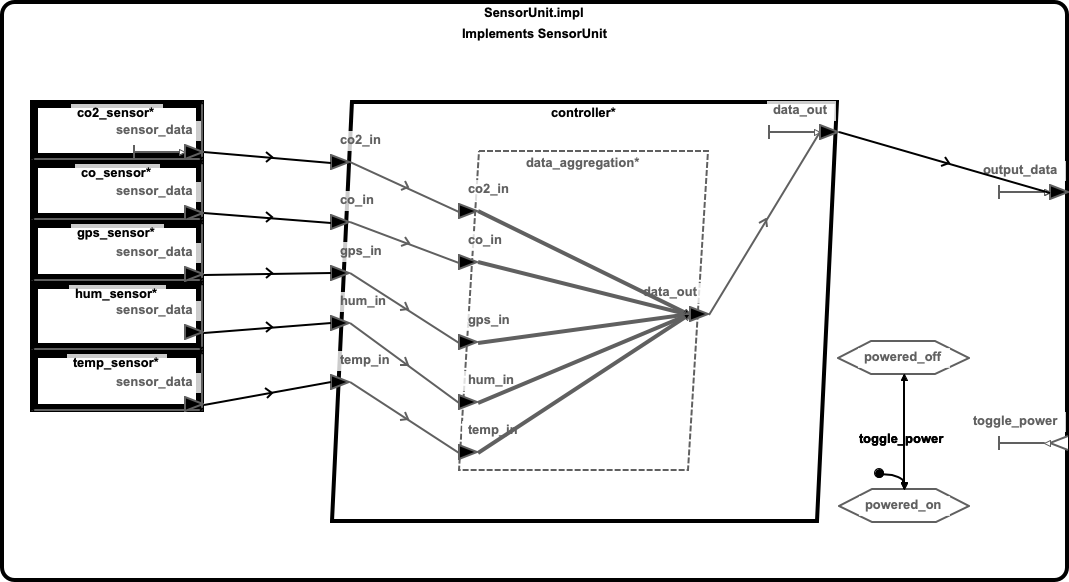
\includegraphics[width=0.9\textwidth]{SensorUnit}
\end{figure*}

\begin{figure*}[h]
\caption{Structure of the Communication Network}
\label{fig:communicationnetwork}
\centering
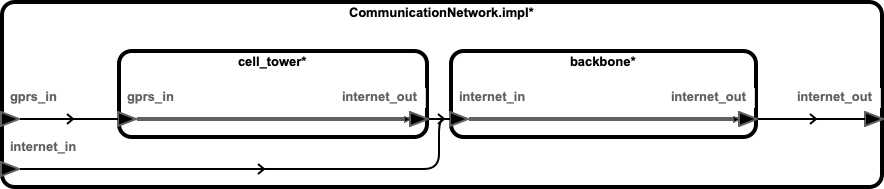
\includegraphics[width=0.9\textwidth]{CommunicationNetwork}
\end{figure*}

\begin{figure}[h]
\caption{Structure of the Control Center}
\label{fig:controlcenter}
\centering
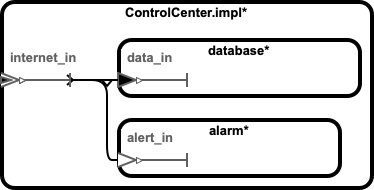
\includegraphics[width=0.45\textwidth]{ControlCenter}
\end{figure}

\subsection{The Sensor Network}

The Sensor Network represents the devices placed within a house or building which together have three purposes: first, collecting environment data that might indicate the presence of a fire; second, sending that data to the Control Center; and third, providing an interface for a local user to monitor the data and configure the sensors. \autoref{fig:sensornetwork} shows the arrangement of the Sensor Network.

To enable this, the Sensor Network is formed by four types of devices:

\begin{enumerate}
	\item Sensor Units, which collect raw environment data;
	\item Communication Units, which receive data from the Sensor Units and forwards it to the relevant destinations;
	\item Mobile Phones, which provide a user interface for monitoring and configuring the other devices; and
	\item one Modem, which connects the Sensor Network to the Internet using wired infrastructure.
\end{enumerate}

The Sensor Units contain five sensors to collect relevant environmental data: ambient temperature, humidity level, carbon monoxide (CO) and dioxide (CO$_2$) concentration, and GPS coordinates.
\autoref{fig:sensorunit} shows the internal structure of a Sensor Unit. 
Since the network can contain multiple Sensor Units (for different rooms inside a house, for example), it is possible to detect precisely where a fire starts and which rooms are affected. 
Sensor Units collect raw environmental data and, using an internal process, combines this information into a single block of data. 
This internal process features a thread that runs at an interval of 100ms to collect and combine data received from sensors.

The combined block of data is then transmitted to the Communication Device using a Zigbee connection. The number of Sensor Units in the network can be configured in a constant value located in \texttt{SensorNetwork.aadl}. Furthermore, the Sensor Units have two modes corresponding to their power status. They can be turned on or off when an appropriate signal is received.

Meanwhile, two Communication Devices exist in the network to collect data from the Sensor Units and transmit it elsewhere. The two devices exist for redundancy, so the system can work even if one of them is faulty. There is also an intercommunication port between the two Communication Devices so they work in a synchronized fashion and can avoid duplicated data. Each Communication Device provides ample communication technologies: 
\begin{itemize}
	\item Zigbee to communicate with the Sensor Units;
	\item Bluetooth to communicate with a Mobile Phone;
	\item Wi-fi and Ethernet to connect to a Modem; and
	\item GPRS for cellular communication.
\end{itemize}

Data collected from the Sensor Units is sent over Bluetooth to a Mobile Phone, which allows user interaction. The Wi-fi, Ethernet and GPRS communication technologies provide both redundancy and flexibility to the system. Ideally, an Ethernet connection provides lower latency communication to the Internet, but Wi-fi and GPRS allow the system to function even if there is a lack of wired infrastructure and permit continuous operation if one is for some reason unavailable.

Aside from providing a bridge between different devices, the Communication Device monitors the sensor data and compares values to a predeterminate threshold. If the temperature, or the CO/CO$_2$ concentration is too high, or the humidity level is too low, an alert signal is sent to the Mobile Phone and to the Control Center, so the necessary measures can be taken.

The Mobile Phone receives data over a Bluetooth connection and displays it in an application. This allows the user to know the current status of the network, the current and historic sensor readings, and control the power each Sensor Unit. Finally, the Modem receives data from the Communication Devices over Wi-fi or Ethernet and transmits packets to the Control Center over the Internet.

The Sensor Network as a whole has two ports to connect to the outside world: one represents a wired connection attached to the Modem, while another shows the cellular GPRS signal sent and received directly by the Communication Device.

\subsection{The Communication Network and the Control Center}

During the development of our model, emphasis was put on the Sensor Network, which we considered the most interesting and complex section of the system. Therefore, the Communication Network and Control Center are rather simple in comparison.

The Communication Network is formed by a Cell Tower, which receives a GPRS signal from the Communication Device and forwards it to the Internet Backbone. The Backbone itself receives wired signal from the Modem or the Cell Tower and abstracts the general Internet infrastructure. \autoref{fig:communicationnetwork} shows the structure of the Communication Network.

The Control Center is the final destination of the sensor readings. It contains a Database, which stores the sensor history for analysis, and an Alarm, which receives an alert signal sent from the Communication Device. With this signal, the designated authorities can dispatch emergency services to the precise location of the fire within a matter of seconds. The Alarm's possible states are modeled as modes: it can either be ringing or not, and switching between modes depends on a signal sent from the Communication Device. \autoref{fig:communicationnetwork} shows the structure of the control center.

\subsection{Auxiliary items}

To help with the structure of the model, a property set and two data types were defined.

The property set allows us to define custom attributes attached to components in the system. 
In it, we defined custom units for data captured by the sensors: temperature is measured in degrees celsius (\degree C), 
humidity is measured in grams per cubic meter (gpm$^3$), 
CO and CO$_2$ concentration is measured in parts per million (ppm) and 
GPS coordinates are tuples of latitude and longitude. 
Each sensor has one or more properties representing the data captured by it.

The data types allow us to analyze the system considering the byte size of data sent through its connections. In our system, each sensor reading can have up to 16 bytes; thus, once the data from the five types of sensors is aggregated and sent through the network, it can be up to 80 bytes of data.

Our analysis is concerned with the connection latency between pairs of components and, therefore, does not suffer influence from the information in the property set and data types.

%\limit{6}

 
\section{Part 2 -- Alternative Architecture and Analysis}

\subsection{Alternative Architecture}

As an alternative to the previously proposed model, we developed a model of a system that functions without the Communication Devices.
For this, the Sensor Units received additional communication capabilities (Bluetooth, wi-fi and GPRS) and the Sensor Network was restructured.

The goal of this alternative is to reduce overall latency by reducing the number of hops data needs to take.
The disadvantage of this approach is that the Sensor Units could become more expensive to produce and the ability to send data over a wired connection is lost.

The remainder of the system remains intact. 

\begin{figure}[h]
\caption{Structure of the alternative Sensor Network}
\label{fig:sensornetworkalt}
\centering
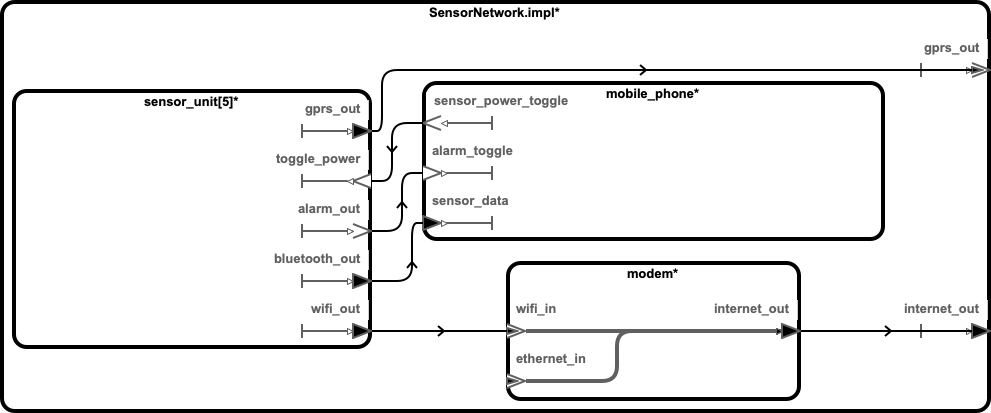
\includegraphics[width=0.45\textwidth]{SensorNetworkAlt}
\end{figure}

\begin{figure}[h]
\caption{Internal structure of an alternative Sensor Unit}
\label{fig:sensorunitalt}
\centering
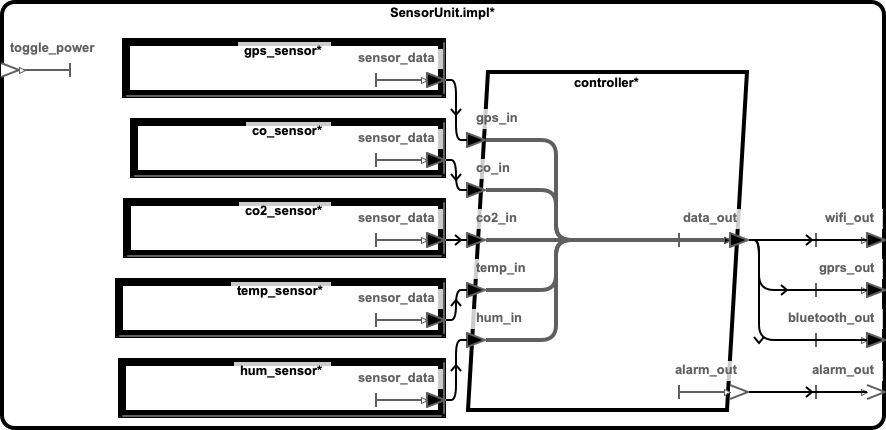
\includegraphics[width=0.45\textwidth]{SensorUnitAlt}
\end{figure}

\subsection{Architectural Analysis}

The AADL model allows us to perform several types of analyses on the system. For the purposes of this assignment, we decided to focus on the flow latency analysis, which seems particularly relevant in the context of a fire alarm system. When it comes to emergencies, response time is crucial, and the system latency can directly impact the agility of emergency services.

In order to perform this analysis, we added flow sources, sinks and paths to our AADL model. Devices that produce data are flow sources, and devices which consume data are flow sinks. Other devices, which only transcode and transmit data, are flow paths. 

Since our system has three primary levels of abstraction, flow sources, sinks and paths had to be added in each one. For example: a Sensor device is a flow source within the context of a Sensor Unit, but the Sensor Unit is the flow source within the context of the Sensor Network, which is itself a flow source within the context of the whole system.

A similar structure applies to flow sinks and paths, which are also present within several layers. Once all sources, sinks and paths are defined, an *end to end flow* is declared, allowing us to perform flow latency analysis on the pairs of sources and sinks are interesting to us.

Since we do not have real world latency values for each communication technology within this context, path latencies were estimated according to general specifications of each technology.

\subsection{Results}

\autoref{fig:rplot02} shows the results of the flow latency analysis, with the minimum and maximum latencies in each flow. The end to end flows analyzed are as follows:

\begin{itemize}
	\item \texttt{etef\_sensor\_phone} and \texttt{etef\_sensor\_phone2}: measure the time it takes for sensor data to reach a Mobile Phone using the first and second Communication Devices, respectively;
	\item \texttt{etef\_sensor\_alarm\_phone} and \texttt{etef\_sensor\_alarm2\_phone}: measure the time it takes for an alert signal produced by the first and second Communication Devices, respectively, to reach a Mobile Phone;
	\item \texttt{etef\_gprs\_db}, \texttt{etef\_ethernet\_db} and \texttt{etef\_wifi\_db}: measure the time it takes for sensor data to reach the Database in the Control Center, for each communication technology; and
	\item \texttt{etef\_gprs\_alarm}, \texttt{etef\_ethernet\_alarm} and \texttt{etef\_wifi\_alarm}: measure the time it takes for an alert signal produced by a Communication Device to reach the Alarm in the Control Center, for each communication technology.
\end{itemize}

\begin{figure}[h]
\caption{Results of the flow latency analysis}
\label{fig:rplot02}
\centering
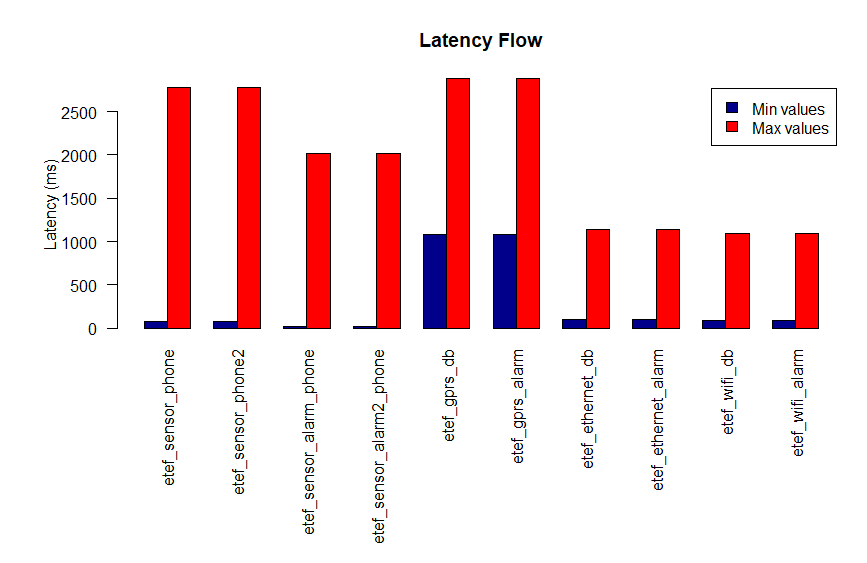
\includegraphics[width=0.45\textwidth]{Rplot02}
\end{figure}

As we can see, there tends to be a large difference between the minimum and maximum latencies, caused by the variable latency in the communication methods and also by the processing time of the data combination thread. Since the thread runs at an interval of 100ms, in the best-case scenario, data reaches the thread immediately before it is executed. On the other hand, if it reaches the thread shortly after execution, the data will only be sent in the next execution 100ms later.

Additionally, we can see that GPRS is the only communication technology with notably greater latency. GPRS signal is sent directly from a Communication Device to a Cell Tower, but it is a slower communication method in general.

Furthermore, an analysis was performed in order to find which ports are used more frequently as flow source or sinks, showing which components are considered crucial to the functioning of the system. \autoref{fig:source} shows the number of times ports are used as flow sources; while \autoref{fig:sink} shows the number of times ports are used as flow sinks.

\begin{figure}[h]
\caption{Ports used as flow sources}
\label{fig:source}
\centering
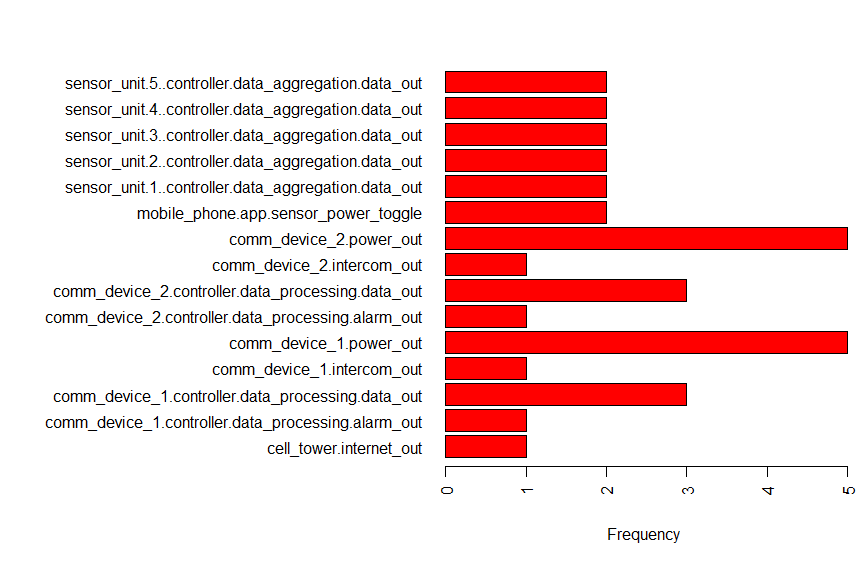
\includegraphics[width=0.45\textwidth]{source}
\end{figure}

\begin{figure}[h]
\caption{Ports used as flow sinks}
\label{fig:sink}
\centering
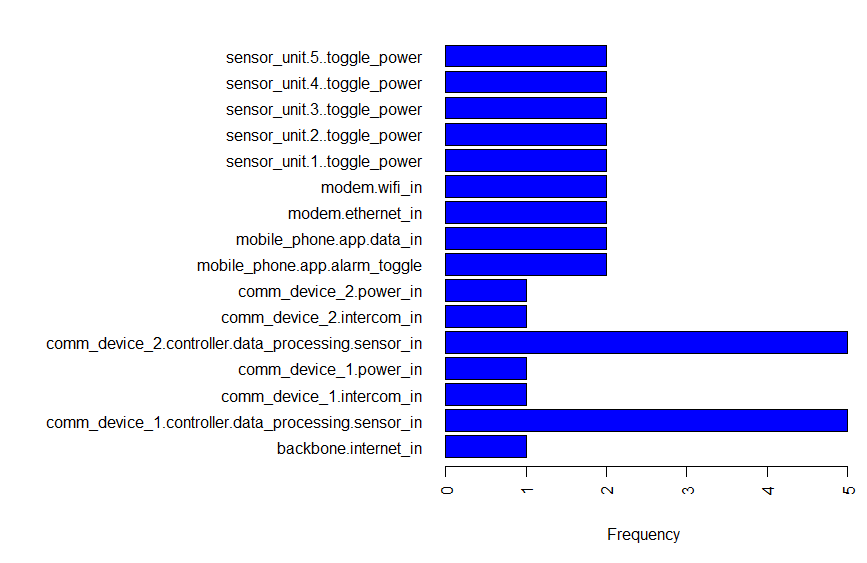
\includegraphics[width=0.45\textwidth]{sink}
\end{figure}


In comparison, \autoref{fig:rplot03} shows the results of the flow latency analysis for the alternative model proposed, with the following flows:

\begin{itemize}
	\item \texttt{etef\_sensor\_phone} and \texttt{etef\_sensor\_alarm\_phone}: measure the time it takes for sensor data or an alert signal to reach a Mobile Phone, respectively;
	\item \texttt{etef\_gprs\_db} and \texttt{etef\_wifi\_db}: measure the time it takes for sensor data to reach the Database in the Control Center, for each communication technology;
	\item \texttt{etef\_gprs\_alarm} and \texttt{etef\_wifi\_alarm}: measure the time it takes for an alert signal produced by a Sensor Unit to reach the Database in the Control Center, for each communication technology;
\end{itemize}

We can see that, by reducing the number of hops in the path, the maximum latencies are much lower. Curiously, with this approach, the GPRS method is faster than Wi-fi, because it avoids the necessity of going through the modem.

\begin{figure}[h]
\caption{Results of the flow latency analysis}
\label{fig:rplot03}
\centering
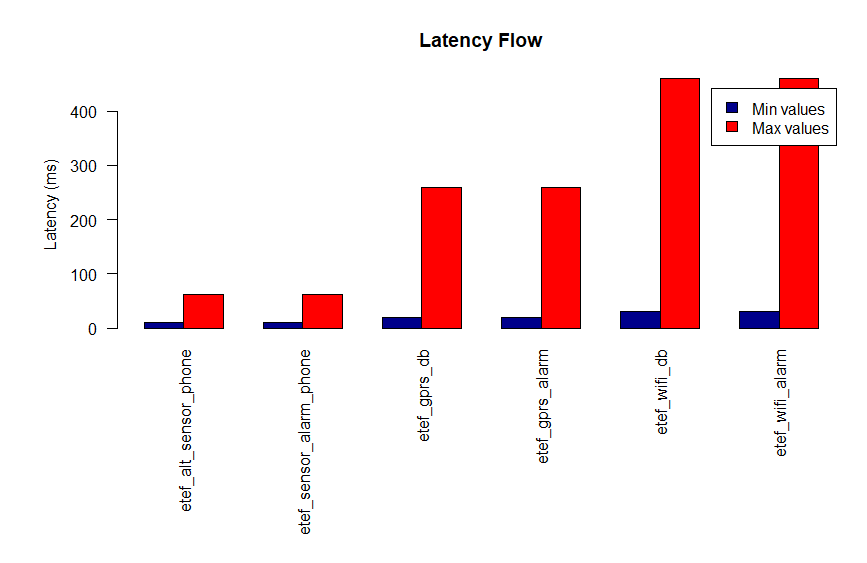
\includegraphics[width=0.45\textwidth]{Rplot03}
\end{figure}

%\limit{6}
\section{Part 3 -- Acceleo}

\subsection{Definition of the Acceleo Program}

Describe how you developed your Acceleo program.

\subsection{Example of output}

Show and discuss the output produced by your Acceleo program.

\limit{6}


\section{Conclusions}\label{sec:conclusions}

One brief paragraph for summarizing the main findings of the assignment.

One brief paragraph about the possible extensions of the performed assignment (imagine that other 3 teams will be assigned to the extension of your experiment).    

\bibliographystyle{IEEEtran}
\bibliography{references}

\end{document}
